\begin{frame}
	\myheading{Module 11.4 : CNNs (success stories on ImageNet)}
\end{frame}

%%%%%%%%%%%%%%%%%%%%%%%%%%%%%%%%%%%%%%%%%%%%%%%%%%%%%%%%%%%%%%%%%%%%%%%%%%%%%%%%%%%%%%%%%

\begin{frame}
	\begin{block}{ImageNet Success Stories(roadmap for rest of the talk)}
		\onslide<1-3>{
			\begin{itemize}
				\justifying
				\item <1-> AlexNet
				\item <2-> ZFNet
				\item <3-> VGGNet
			\end{itemize}
		}
	\end{block}
\end{frame}

%%%%%%%%%%%%%%%%%%%%%%%%%%%%%%%%%%%%%%%%%%%%%%%%%%%%%%%%%%%%%%%%%%%%%%%%%%%%%%%%%%%%%%%%%

\begin{frame}
	%\centering
	\begin{flushleft}
		\begin{tikzpicture}%[scale=0.9,remember picture,overlay,shift={(current page.south west)}] 
 
	\pgfsetxvec{\pgfpoint{1cm}{0cm}}
	\pgfsetyvec{\pgfpoint{0cm}{1cm}}
	\pgfsetzvec{\pgfpoint{-0.707cm}{.707cm}}  
    
	\onslide<1->{
		\draw[black!50] (1,2) -- (13,2);
		\mylabel{(2.5,2,0)}{blue!30}{0.4}{-4}{0}{ILSVRC'10}{28.2}{}
		\only<9>{
			\mylabel{(2.5,2,0)}{blue!30}{0.4}{-4}{0}{ILSVRC'10}{28.2}{}
		}
	}
    
	\onslide<2->{
		\mylabel{(4,2,0)}{blue!30}{0.4}{-3.66}{0}{ILSVRC'11}{25.8}{}
		\only<9>{
			\mylabel{(4,2,0)}{blue!30}{0.4}{-3.66}{0}{ILSVRC'11}{25.8}{}
		}
	}
    
	\onslide<3->{
		\mylabel{(5.5,2,0)}{blue!30}{0.4}{-2.33}{0}{ILSVRC'12}{16.4}{AlexNet}
		\only<9>{
			\mylabel{(5.5,2,0)}{green!30}{0.4}{-2.33}{0}{ILSVRC'12}{16.4}{AlexNet}
		}
	}
    
	\onslide<4->{
		\mylabel{(7,2,0)}{blue!30}{0.4}{-1.66}{0}{ILSVRC'13}{11.7}{ZFNet}
		\only<9>{
			\mylabel{(7,2,0)}{green!30}{0.4}{-1.66}{0}{ILSVRC'13}{11.7}{ZFNet}
		}
	}
    
	\onslide<5->{
		\mylabel{(8.5,2,0)}{blue!30}{0.4}{-1.04}{0}{ILSVRC'14}{7.3}{VGG}
		\only<9>{
			\mylabel{(8.5,2,0)}{green!30}{0.4}{-1.04}{0}{ILSVRC'14}{7.3}{VGG}
		}
	}
    
	\onslide<6->{
		\mylabel{(10,2,0)}{blue!30}{0.4}{-0.95}{0}{ILSVRC'14}{6.7}{GoogleNet}
		\only<9>{
			\mylabel{(10,2,0)}{green!30}{0.4}{-0.95}{0}{ILSVRC'14}{6.7}{GoogleNet}
		}
	}
    
	\onslide<7->{
		\mylabel{(11.5,2,0)}{blue!30}{0.4}{-0.5}{0}{ILSVRC'15}{3.57}{ResNet}
		\only<9>{
			\mylabel{(11.5,2,0)}{green!30}{0.4}{-0.5}{0}{ILSVRC'15}{3.57}{ResNet}
		}
	}
    
	\onslide<8->{
		\mybox{(2,2.5,0)}{pink!10}{-2.1}{-0.4}{0}{shallow}
     
		\mybox{(4.7,2.5,0)}{pink!10}{-1.2}{-0.4}{0}{8 layers}
     
		\mybox{(6.2,2.5,0)}{pink!10}{-1.2}{-0.4}{0}{8 layers}
     
		\mybox{(7.7,3.5,0)}{pink!10}{-1.2}{-0.4}{0}{19 layers}
     
		\mybox{(9.2,3.5,0)}{pink!10}{-1.2}{-0.4}{0}{22 layers}
     
		\mybox{(10.7,5.5,0)}{pink!10}{-1.2}{-0.4}{0}{152 layers}
     
		\triangle{2.2}{2}{orange!50}
		\triangle{3.7}{2.02}{orange!50}
		\triangle{5.2}{2.2}{orange!50}
		\triangle{6.7}{2.2}{orange!50}
		\triangle{8.2}{2.5}{orange!50}
		\triangle{9.7}{2.6}{orange!50}
		\triangle{11.2}{5.2}{orange!50}
     
		\draw[dashed,draw=orange!50,line width=0.7] (2.3,2.1) -- (3.8,2.12);
		\draw[dashed,draw=orange!50,line width=0.7] (3.8,2.12) -- (5.3,2.3);
		\draw[dashed,draw=orange!50,line width=0.7] (5.3,2.3) -- (6.8,2.3);
		\draw[dashed,draw=orange!50,line width=0.7] (6.8,2.3) -- (8.3,2.6);
		\draw[dashed,draw=orange!50,line width=0.7] (8.3,2.6) -- (9.8,2.7);
		\draw[dashed,draw=orange!50,line width=0.7] (9.8,2.7) -- (11.3,5.3);
	}
    
\end{tikzpicture}
	\end{flushleft}
\end{frame}

%%%%%%%%%%%%%%%%%%%%%%%%%%%%%%%%%%%%%%%%%%%%%%%%%%%%%%%%%%%%%%%%%%%%%%%%%%%%%%%%%%%%%%%%%

\begin{frame}
	\begin{block}{ImageNet Success Stories(roadmap for rest of the talk)}
		\onslide<1>{
			\begin{itemize}
				\justifying
				\item <1-> \textcolor{red}{AlexNet}
				\item <1-> ZFNet
				\item <1-> VGGNet
				      
			\end{itemize}
		}
	\end{block}
\end{frame}

%%%%%%%%%%%%%%%%%%%%%%%%%%%%%%%%%%%%%%%%%%%%%%%%%%%%%%%%%%%%%%%%%%%%%%%%%%%%%%%%%%%%%%%%%

\begin{frame}
	\begin{center}
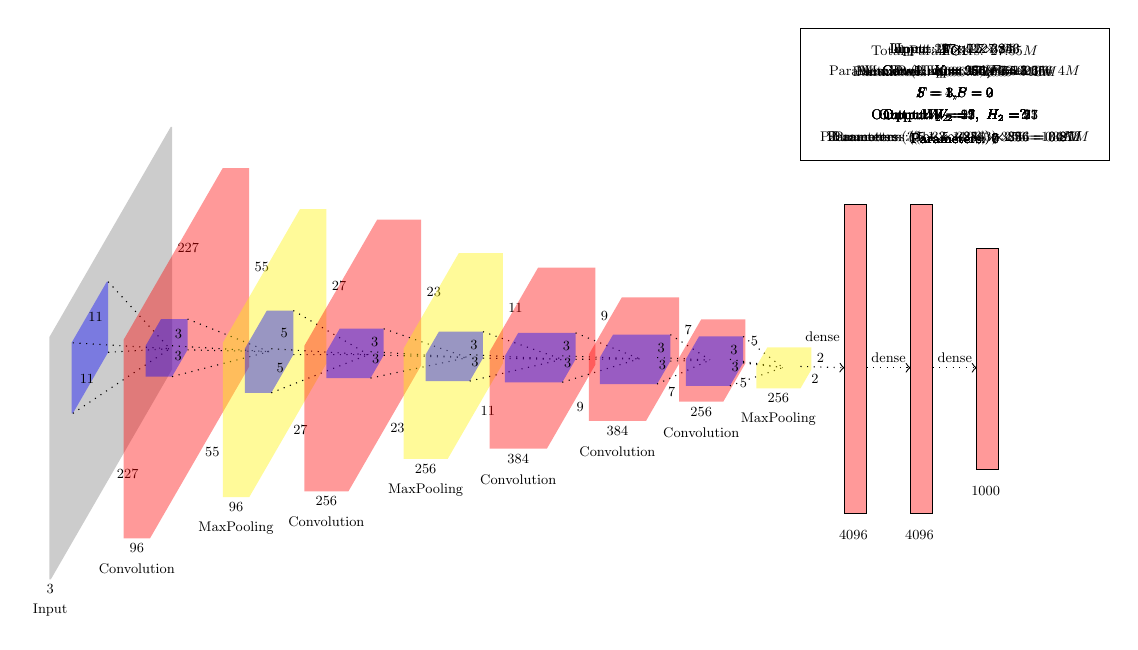
\begin{tikzpicture}[scale=0.56,transform shape]

\pgfsetxvec{\pgfpoint{1cm}{0cm}}
\pgfsetyvec{\pgfpoint{0cm}{1cm}}
\pgfsetzvec{\pgfpoint{-.5cm}{-.866cm}}

\def\cuboid#1#2#3#4#5{
\begin{scope}
\edef\mycolor{#2}
\edef\depth{#3}
\edef\height{#4}
\edef\width{#5}
\draw[black,fill=\mycolor, fill opacity=0.4, text opacity=1] #1 -- ++(-\depth,0,0) -- ++(0,-\height,0) -- ++(\depth,0,0) -- cycle #1 -- ++(0,0,-\width) -- ++(0,-\height,0) -- ++(0,0,\width) -- cycle  #1 -- ++(-\depth,0,0) -- ++(0,0,-\width) -- ++(\depth,0,0) -- cycle;
\end{scope}
}

\def\cuboidlabel#1#2#3#4#5#6#7#8{
\begin{scope}
\edef\mycolor{#2}
\edef\depth{#3}
\edef\height{#4}
\edef\width{#5}
\edef\depthlabel{#6}
\edef\heightlabel{#7}
\edef\widthlabel{#8}
\draw[draw=none,fill=\mycolor, fill opacity=0.4, text opacity=1] #1 -- ++(-\depth,0,0) -- ++(0,-\height,0) -- ++(\depth,0,0) node[black,pos=0.5,below] {\small \depthlabel} -- cycle #1 -- ++(0,0,-\width) -- ++(0,-\height,0) node[black,pos=0.5,right] {\small \heightlabel} -- ++(0,0,\width)  node[black,pos=0.5,below,right] {\small \widthlabel} -- cycle  #1 -- ++(-\depth,0,0) -- ++(0,0,-\width) -- ++(\depth,0,0) -- cycle;
\end{scope}
}

\def\kernel#1#2#3#4#5#6{
\begin{scope}
\edef\mycolor{#2}
\edef\depth{#3}
\edef\height{#4}
\edef\width{#5}
\draw[black,fill=\mycolor, fill opacity=0.4, text opacity=1] #1 -- ++(-\depth,0,0) -- ++(0,-\height,0) -- ++(\depth,0,0) -- cycle #1 -- ++(0,0,-\width) -- ++(0,-\height,0) -- ++(0,0,\width) -- cycle  #1 -- ++(-\depth,0,0) -- ++(0,0,-\width) -- ++(\depth,0,0) -- cycle;

\draw[dotted] #1 -- #6 #1++(0,0,-\width) -- #6 #1++(0,-\height,0) -- #6 #1++(0,-\height,-\width) -- #6;

\end{scope}
}

\def\kernellabel#1#2#3#4#5#6#7#8#9{
%#6 is target pixel
\begin{scope}
\edef\mycolor{#2}
\edef\depth{#3}
\edef\height{#4}
\edef\width{#5}
\edef\depthlabel{#7}
\edef\heightlabel{#8}
\edef\widthlabel{#9}
\draw[draw=none,fill=\mycolor, fill opacity=0.4, text opacity=1] #1 -- ++(-\depth,0,0) -- ++(0,-\height,0) -- ++(\depth,0,0) -- cycle #1 -- ++(0,0,-\width) -- ++(0,-\height,0) node[pos=0.5,left] {\small \heightlabel} -- ++(0,0,\width)  node[pos=0.6,above] {\small \widthlabel} -- cycle  #1 -- ++(-\depth,0,0) -- ++(0,0,-\width) -- ++(\depth,0,0) -- cycle;

\draw[dotted] #1 -- #6 #1++(0,0,-\width) -- #6 #1++(0,-\height,0) -- #6 #1++(0,-\height,-\width) -- #6;

\end{scope}
}

\cuboid{(24,7,0)}{white}{7}{3}{0}{256}{2}{2}

%alexnet
\onslide<1->{
\cuboidlabel{(0,0,0)}{gray}{0.03}{5.5}{5.5}{3}{227}{227}
\node (a) at (-0.015,-6.2,0) {\small Input};
}
\onslide<2->{
\kernellabel{(0,-1,-1)}{blue}{0.03}{1.6}{1.6}{(1.7,-2,-2)}{3}{11}{11}
}
\onslide<2-4>{
\node (a) at (24-7*0.5,7-0.5) {\small Input: $227 \times 227 \times 3$};
\node (a) at (24-7*0.5,7-1) {\small Conv1: $K=96$,$F=11$};
\node (a) at (24-7*0.5,7-1.5) {\small $S=4$,$P=0$};
\onslide<2>{\node (a) at (24-7*0.5,7-2) {\small Output:$W_2=?,\ H_2=?$};}
\onslide<3-4>{\node (a) at (24-7*0.5,7-2) {\small Output:$W_2=55,\ H_2=55$};}
\onslide<2-3>{\node (a) at (24-7*0.5,7-2.5) {\small Parameters: $?$};}
\onslide<4>{\node (a) at (24-7*0.5,7-2.5) {\small Parameters: $(11\times 11 \times 3)\times 96 = 34K$};}
}

\onslide<3->{
\cuboidlabel{(2,-0.5,-0.5)}{red}{0.6}{4.5}{4.5}{96}{55}{55}
\node (a) at (2-0.3,-0.5-4.5-0.7,-0.5) {\small Convolution};
}
\onslide<5->{
\kernellabel{(2,-1.5,-1.5)}{blue}{0.6}{0.7}{0.7}{(3.7,-2.5,-2.5)}{96}{3}{3}
}
%\onslide<4>{
%\node (a) at (2-0.3+1,-6.7,-0.5) {\scriptsize $S=2$,$P=0$};
%\node (a) at (2-0.3+1,-7.2,-0.5) {\scriptsize Parameters: 0};
%}

\onslide<5-7>{
\node (a) at (24-7*0.5,7-1) {\small Max Pool Input: $55 \times 55 \times 96$};
\node (a) at (24-7*0.5,7-1.5) {\small $F=3$,$S=2$};
\onslide<5>{\node (a) at (24-7*0.5,7-2) {\small Output:$W_2=?,\ H_2=?$};}
\onslide<6-7>{\node (a) at (24-7*0.5,7-2) {\small Output:$W_2=27,\ H_2=27$};}
\onslide<5-6>{\node (a) at (24-7*0.5,7-2.5) {\small Parameters: $?$};}
\onslide<7>{\node (a) at (24-7*0.5,7-2.5) {\small Parameters: $0$};}
}


\onslide<6->{
\cuboidlabel{(4,-1,-1)}{yellow}{0.6}{3.5}{3.5}{96}{27}{27}
\node (a) at (4-0.3,-1-3.5-0.7,-1) {\small MaxPooling};
}
\onslide<8->{
\kernellabel{(4,-2,-2)}{blue}{0.6}{1}{1}{(5.7,-3,-3)}{96}{5}{5}
}
%\onslide<6>{
%\node (a) at (4-0.3+1,-6.7,-1) {\scriptsize $S=1$,$P=0$};
%\node (a) at (4-0.3+1,-7.2,-1) {\scriptsize Parameters: $(5\times 5 \times 96)\times 256 = K$};
%}

\onslide<8-10>{
\node (a) at (24-7*0.5,7-0.5) {\small Input: $27 \times 27 \times 96$};
\node (a) at (24-7*0.5,7-1) {\small Conv1: $K=256$,$F=5$};
\node (a) at (24-7*0.5,7-1.5) {\small $S=1$,$P=0$};
\onslide<8>{\node (a) at (24-7*0.5,7-2) {\small Output:$W_2=?,\ H_2=?$};}
\onslide<9-10>{\node (a) at (24-7*0.5,7-2) {\small Output:$W_2=23,\ H_2=23$};}
\onslide<8-9>{\node (a) at (24-7*0.5,7-2.5) {\small Parameters: $?$};}
\onslide<10>{\node (a) at (24-7*0.5,7-2.5) {\small Parameters: $(5\times 5 \times 96)\times 256=0.6M$};}
}

\onslide<9->{
\cuboidlabel{(6,-1.5,-1.5)}{red}{1}{3.3}{3.3}{256}{23}{23}
\node (a) at (6-0.5,-1.5-3.3-0.7,-1.5) {\small Convolution};
}
\onslide<11->{
\kernellabel{(6,-2.5,-2.5)}{blue}{1}{0.6}{0.6}{(7.7,-3.5,-3.5)}{256}{3}{3}
}
%\onslide<8>{
%\node (a) at (6-0.5+1,-6.7,-1.5) {\scriptsize $S=2$,$P=0$};
%\node (a) at (6-0.5+1,-7.2,-1.5) {\scriptsize Parameters: 0};
%}

\onslide<11-13>{
\node (a) at (24-7*0.5,7-1) {\small Max Pool Input: $23 \times 23 \times 256$};
\node (a) at (24-7*0.5,7-1.5) {\small $F=3$,$S=2$};
\onslide<11>{\node (a) at (24-7*0.5,7-2) {\small Output:$W_2=?,\ H_2=?$};}
\onslide<12-13>{\node (a) at (24-7*0.5,7-2) {\small Output:$W_2=11,\ H_2=11$};}
\onslide<11-12>{\node (a) at (24-7*0.5,7-2.5) {\small Parameters: $?$};}
\onslide<13>{\node (a) at (24-7*0.5,7-2.5) {\small Parameters: $0$};}
}


\onslide<12->{
\cuboidlabel{(8,-2,-2)}{yellow}{1}{2.5}{2.5}{256}{11}{11}
\node (a) at (8-0.5,-2-2.5-0.7,-2) {\small MaxPooling};
}
\onslide<14->{
\kernellabel{(8,-3,-3)}{blue}{1}{0.6}{0.6}{(9.7,-3.8,-3.8)}{256}{3}{3}
}
%\onslide<10>{
%\node (a) at (8-0.5+1,-6.7,-2) {\scriptsize $S=1$,$P=0$};
%\node (a) at (8-0.5+1,-7.2,-2) {\scriptsize Parameters: $(3\times 3 \times 256)\times 384 = K$};
%}
\onslide<14-16>{
\node (a) at (24-7*0.5,7-0.5) {\small Input: $11 \times 11 \times 256$};
\node (a) at (24-7*0.5,7-1) {\small Conv1: $K=384$,$F=3$};
\node (a) at (24-7*0.5,7-1.5) {\small $S=1$,$P=0$};
\onslide<14>{\node (a) at (24-7*0.5,7-2) {\small Output:$W_2=?,\ H_2=?$};}
\onslide<15-16>{\node (a) at (24-7*0.5,7-2) {\small Output:$W_2=9,\ H_2=9$};}
\onslide<14-15>{\node (a) at (24-7*0.5,7-2.5) {\small Parameters: $?$};}
\onslide<16>{\node (a) at (24-7*0.5,7-2.5) {\small Parameters: $(3\times 3 \times 256)\times 384=0.8M$};}
}

\onslide<15->{
\cuboidlabel{(10,-2.5,-2.5)}{red}{1.3}{2.2}{2.2}{384}{9}{9}
\node (a) at (10-0.65,-2.5-2.2-0.7,-2.5) {\small Convolution};
}
\onslide<17->{
\kernellabel{(10,-3.2,-3.2)}{blue}{1.3}{0.6}{0.6}{(11.5,-3.7,-3.7)}{384}{3}{3}
}
%\onslide<12>{
%\node (a) at (10-0.65+1,-6.7,-2.5) {\scriptsize $S=1$,$P=0$};
%\node (a) at (10-0.65+1,-7.2,-2.5) {\scriptsize Parameters: $(3\times 3 \times 384)\times 384 = K$};
%}
\onslide<17-19>{
\node (a) at (24-7*0.5,7-0.5) {\small Input: $9 \times 9 \times 384$};
\node (a) at (24-7*0.5,7-1) {\small Conv1: $K=384$,$F=3$};
\node (a) at (24-7*0.5,7-1.5) {\small $S=1$,$P=0$};
\onslide<17>{\node (a) at (24-7*0.5,7-2) {\small Output:$W_2=?,\ H_2=?$};}
\onslide<18-19>{\node (a) at (24-7*0.5,7-2) {\small Output:$W_2=7,\ H_2=7$};}
\onslide<17-18>{\node (a) at (24-7*0.5,7-2.5) {\small Parameters: $?$};}
\onslide<19>{\node (a) at (24-7*0.5,7-2.5) {\small Parameters:  $(3\times 3 \times 384)\times 384=1.327M$};}
}


\onslide<18->{
\cuboidlabel{(12,-3,-3)}{red}{1.3}{1.5}{1.5}{384}{7}{7}
\node (a) at (12-0.65,-3-1.5-0.7,-3) {\small Convolution};
}
\onslide<20->{
\kernellabel{(12,-3.5,-3.5)}{blue}{1.3}{0.6}{0.6}{(13,-3.9,-3.9)}{384}{3}{3}
}
%\onslide<14>{
%\node (a) at (12-0.65+1,-6.7,-3) {\scriptsize $S=1$,$P=0$};
%\node (a) at (12-0.65+1,-7.2,-3) {\scriptsize Parameters: $(3\times 3 \times 384)\times 256 = K$};
%}
\onslide<20-22>{
\node (a) at (24-7*0.5,7-0.5) {\small Input: $7 \times 7 \times 384$};
\node (a) at (24-7*0.5,7-1) {\small Conv1: $K=256$,$F=3$};
\node (a) at (24-7*0.5,7-1.5) {\small $S=1$,$P=0$};

\onslide<20>{\node (a) at (24-7*0.5,7-2) {\small Output:$W_2=?,\ H_2=?$};}
\onslide<21-22>{\node (a) at (24-7*0.5,7-2) {\small Output:$W_2=5,\ H_2=5$};}
\onslide<20-21>{\node (a) at (24-7*0.5,7-2.5) {\small Parameters: $?$};}
\onslide<22>{\node (a) at (24-7*0.5,7-2.5) {\small Parameters:  $(3\times 3 \times 384)\times 256=0.8M$};}
}

\onslide<21->{
\cuboidlabel{(13.5,-3.5,-3.5)}{red}{1}{1}{1}{256}{5}{5}
\node (a) at (13.5-0.5,-3.5-1-0.7,-3.5) {\small Convolution};
}
\onslide<23->{
\kernellabel{(13.5,-3.8,-3.8)}{blue}{1}{0.6}{0.6}{(14,-5.2,-5.2)}{256}{3}{3}
}
%\onslide<16>{
%\node (a) at (13.5-0.5+1,-6.7,-3.5) {\scriptsize $S=2$,$P=0$};
%\node (a) at (13.5-0.5+1,-7.2,-3.5) {\scriptsize Parameters: 0};
%}
\onslide<23-25>{
\node (a) at (24-7*0.5,7-1) {\small Max Pool Input: $5 \times 5 \times 256$};
\node (a) at (24-7*0.5,7-1.5) {\small $F=3$,$S=2$};
\onslide<23>{\node (a) at (24-7*0.5,7-2) {\small Output:$W_2=?,\ H_2=?$};}
\onslide<24-25>{\node (a) at (24-7*0.5,7-2) {\small Output:$W_2=2,\ H_2=2$};}
\onslide<23-24>{\node (a) at (24-7*0.5,7-2.5) {\small Parameters: $?$};}
\onslide<25>{\node (a) at (24-7*0.5,7-2.5) {\small Parameters:  $0$};}
}


\onslide<24->{
\cuboidlabel{(14.5,-5,-5)}{yellow}{1}{0.5}{0.5}{256}{2}{2}
\node (a) at (14.5-0.5,-5-0.5-0.7,-5) {\small MaxPooling};
}

\onslide<26>{
\node (a) at (24-7*0.5,7-0.5) {\small FC1};
\node (a) at (24-7*0.5,7-1) {\small Parameters: $(2\times 2 \times 256)\times 4096 = 4M$};
}

\onslide<26->{
\draw[dotted,->] (14.5,-5,-5) -- (18,-0.7,0);
\node (a) at (17.5,0,0) {\small dense};
\cuboid{(18.5,3,0)}{red}{0.5}{7}{0}{256}{2}{2}
\node (a) at (18.2,-4.5,0) {\small 4096};
}

\onslide<27>{
\node (a) at (24-7*0.5,7-0.5) {\small FC1};
\node (a) at (24-7*0.5,7-1) {\small Parameters: $4096 \times 4096 = 16M$};
}

\onslide<27->{
\draw[dotted,->] (18.5,-0.7,0) -- (19+0.5,-0.7,0) node[pos=0.5,above] {\small dense};
\cuboid{(19.5+0.5,3,0)}{red}{0.5}{7}{0}{256}{2}{2}
\node (a) at (19.2+0.5,-4.5,0) {\small 4096};
}

\onslide<28->{
\draw[dotted,->] (19.5+0.5,-0.7,0) -- (20+1,-0.7,0) node[pos=0.5,above] {\small dense};
\cuboid{(20.5+1,2,0)}{red}{0.5}{5}{0}{256}{2}{2}
\node (a) at (20.2+1,-3.5,0) {\small 1000};
}


\onslide<28>{
\node (a) at (24-7*0.5,7-0.5) {\small FC1};
\node (a) at (24-7*0.5,7-1) {\small Parameters: $4096 \times 1000 = 4M$};
}
\onslide<29>{
\node (a) at (24-7*0.5,7-0.5) {\small Total Parameters: $27.55M$};
}





\end{tikzpicture}
\end{center}


\end{frame}

%%%%%%%%%%%%%%%%%%%%%%%%%%%%%%%%%%%%%%%%%%%%%%%%%%%%%%%%%%%%%%%%%%%%%%%%%%%%%%%%%%%%%%%%%

\begin{frame}
	\begin{columns}
		\column{0.3\textwidth}
		\begin{itemize}
			\justifying
			\item <1-> Let us look at the connections in the fully connected layers in more detail
			\item <2-> We will first stretch out the last conv or maxpool layer to make it a 1d vector
			\item <3-> This 1d vector is then densely connected to other layers just as in a regular feedforward neural network 
		\end{itemize}
		
		\column{0.7\textwidth}
		\begin{overlayarea}{\textwidth}{\textheight}
			\begin{center}
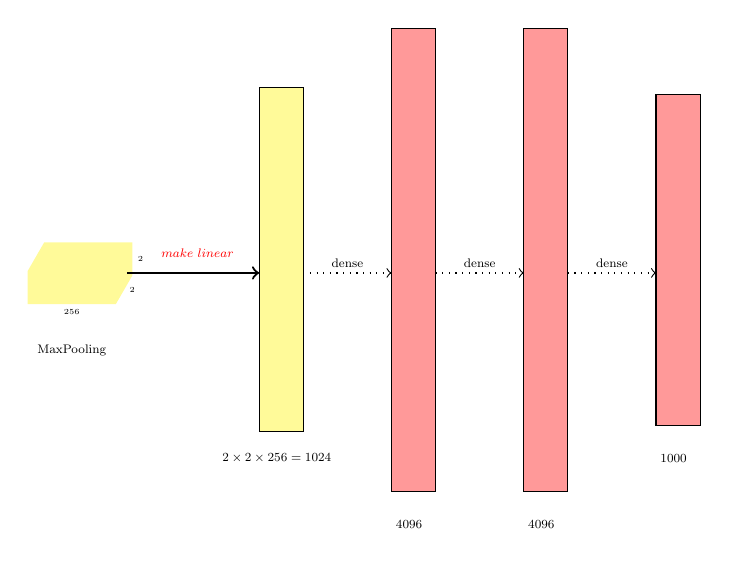
\begin{tikzpicture}[scale=0.56,transform shape]

\pgfsetxvec{\pgfpoint{2cm}{0cm}}
\pgfsetyvec{\pgfpoint{0cm}{1.5cm}}
\pgfsetzvec{\pgfpoint{-.5*1.5cm}{-.866*1.5cm}}

\def\cuboid#1#2#3#4#5{
\begin{scope}
\edef\mycolor{#2}
\edef\depth{#3}
\edef\height{#4}
\edef\width{#5}
\draw[black,fill=\mycolor, fill opacity=0.4, text opacity=1] #1 -- ++(-\depth,0,0) -- ++(0,-\height,0) -- ++(\depth,0,0) -- cycle #1 -- ++(0,0,-\width) -- ++(0,-\height,0) -- ++(0,0,\width) -- cycle  #1 -- ++(-\depth,0,0) -- ++(0,0,-\width) -- ++(\depth,0,0) -- cycle;
\end{scope}
}

\def\cuboidlabel#1#2#3#4#5#6#7#8{
\begin{scope}
\edef\mycolor{#2}
\edef\depth{#3}
\edef\height{#4}
\edef\width{#5}
\edef\depthlabel{#6}
\edef\heightlabel{#7}
\edef\widthlabel{#8}
\draw[draw=none,fill=\mycolor, fill opacity=0.4, text opacity=1] #1 -- ++(-\depth,0,0) -- ++(0,-\height,0) -- ++(\depth,0,0) node[black,pos=0.5,below] {\tiny \depthlabel} -- cycle #1 -- ++(0,0,-\width) -- ++(0,-\height,0) node[black,pos=0.5,right] {\tiny \heightlabel} -- ++(0,0,\width)  node[black,pos=0.5,below,right] {\tiny \widthlabel} -- cycle  #1 -- ++(-\depth,0,0) -- ++(0,0,-\width) -- ++(\depth,0,0) -- cycle;
\end{scope}
}

\def\kernel#1#2#3#4#5#6{
\begin{scope}
\edef\mycolor{#2}
\edef\depth{#3}
\edef\height{#4}
\edef\width{#5}
\draw[black,fill=\mycolor, fill opacity=0.4, text opacity=1] #1 -- ++(-\depth,0,0) -- ++(0,-\height,0) -- ++(\depth,0,0) -- cycle #1 -- ++(0,0,-\width) -- ++(0,-\height,0) -- ++(0,0,\width) -- cycle  #1 -- ++(-\depth,0,0) -- ++(0,0,-\width) -- ++(\depth,0,0) -- cycle;

\draw[dotted] #1 -- #6 #1++(0,0,-\width) -- #6 #1++(0,-\height,0) -- #6 #1++(0,-\height,-\width) -- #6;

\end{scope}
}

\def\kernellabel#1#2#3#4#5#6#7#8#9{
%#6 is target pixel
\begin{scope}
\edef\mycolor{#2}
\edef\depth{#3}
\edef\height{#4}
\edef\width{#5}
\edef\depthlabel{#7}
\edef\heightlabel{#8}
\edef\widthlabel{#9}
\draw[draw=none,fill=\mycolor, fill opacity=0.4, text opacity=1] #1 -- ++(-\depth,0,0) -- ++(0,-\height,0) -- ++(\depth,0,0) -- cycle #1 -- ++(0,0,-\width) -- ++(0,-\height,0) node[pos=0.5,left] {\tiny \heightlabel} -- ++(0,0,\width)  node[pos=0.6,above] {\tiny \widthlabel} -- cycle  #1 -- ++(-\depth,0,0) -- ++(0,0,-\width) -- ++(\depth,0,0) -- cycle;

\draw[dotted] #1 -- #6 #1++(0,0,-\width) -- #6 #1++(0,-\height,0) -- #6 #1++(0,-\height,-\width) -- #6;

\end{scope}
}

%\cuboid{(24,7,0)}{white}{7}{3}{0}{256}{2}{2}

%alexnet

\onslide<1->{
\cuboidlabel{(14.5,-5,-5)}{yellow}{1}{0.5}{0.5}{256}{2}{2}
\node (a) at (14.5-0.5,-5-0.5-0.7,-5) {\footnotesize MaxPooling};
}

\onslide<2->{
\draw[thick,->] (16.5,-0.7,0) -- (18,-0.7,0);
\node (a) at (17.3,-0.4,0) {\footnotesize \color{red}{$make\ linear$}};
\cuboid{(18.5,2.1,0)}{yellow}{0.5}{5.2}{0}{256}{2}{2}
\node (a) at (18.2,-3.5,0) {\footnotesize $2\times 2\times 256 = 1024$};
}

\onslide<3->{
\draw[dotted,->] (18.5,-0.7,0) -- (19+0.5,-0.7,0) node[pos=0.5,above] {\footnotesize dense};
\cuboid{(19.5+0.5,3,0)}{red}{0.5}{7}{0}{256}{2}{2}
\node (a) at (19.2+0.5,-4.5,0) {\footnotesize 4096};
}


\onslide<4->{
\draw[dotted,->] (19.5+0.5,-0.7,0) -- (20+1,-0.7,0) node[pos=0.5,above] {\footnotesize dense};
\cuboid{(20.5+1,3,0)}{red}{0.5}{7}{0}{256}{2}{2}
\node (a) at (20.2+1,-4.5,0) {\footnotesize 4096};
}

\onslide<5->{
\draw[dotted,->] (20.5+1,-0.7,0) -- (21.5+1,-0.7,0) node[pos=0.5,above] {\footnotesize dense};
\cuboid{(22+1,2,0)}{red}{0.5}{5}{0}{256}{2}{2}
\node (a) at (21.7+1,-3.5,0) {\footnotesize 1000};
}


\end{tikzpicture}
\end{center}


		\end{overlayarea}
	\end{columns}
\end{frame}

%%%%%%%%%%%%%%%%%%%%%%%%%%%%%%%%%%%%%%%%%%%%%%%%%%%%%%%%%%%%%%%%%%%%%%%%%%%%%%%%%%%%%%%%%

\begin{frame}
	\begin{block}{ImageNet Success Stories(roadmap for rest of the talk)}
		\onslide<1>{
			\begin{itemize}
				\justifying
				\item <1-> \textcolor{red}{AlexNet}
				\item <1-> \textcolor{red}{ZFNet}
				\item <1-> VGGNet
				      
			\end{itemize}
		}
	\end{block}
\end{frame}

%%%%%%%%%%%%%%%%%%%%%%%%%%%%%%%%%%%%%%%%%%%%%%%%%%%%%%%%%%%%%%%%%%%%%%%%%%%%%%%%%%%%%%%%%

\begin{frame}
	\begin{center}
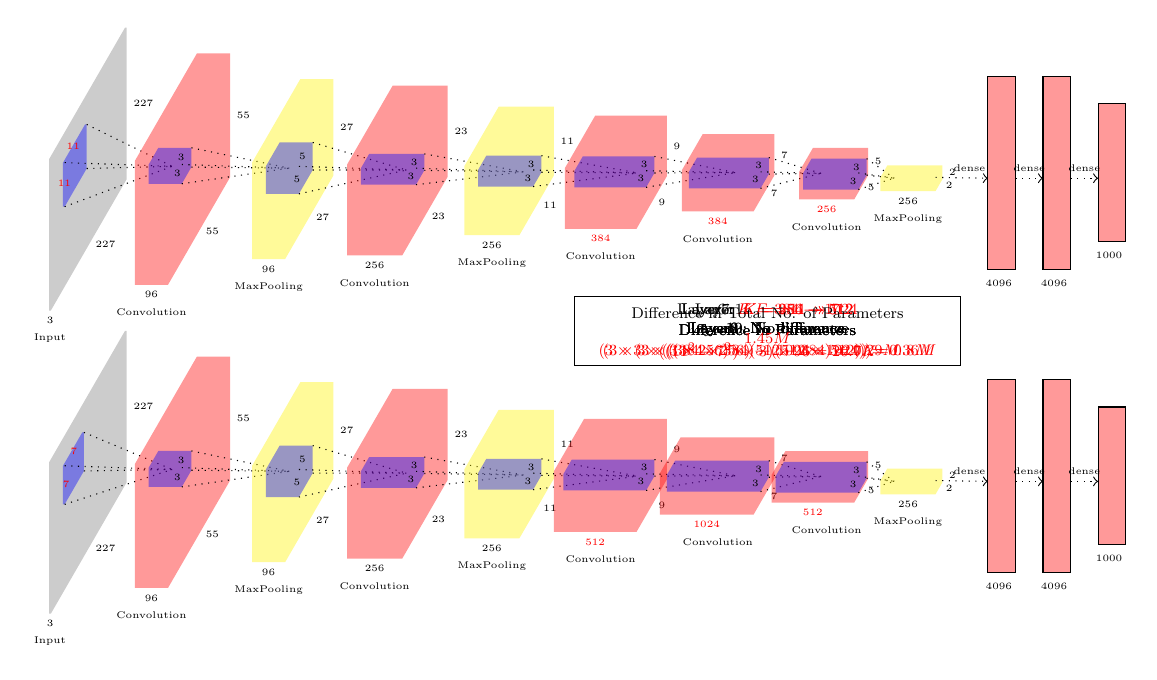
\begin{tikzpicture}[scale=0.7,transform shape]

\pgfsetxvec{\pgfpoint{1cm}{0cm}}
\pgfsetyvec{\pgfpoint{0cm}{0.5*1cm}}
\pgfsetzvec{\pgfpoint{0.5*-.5cm}{0.5*-.866cm}}

\def\cuboid#1#2#3#4#5{
\begin{scope}
\edef\mycolor{#2}
\edef\depth{#3}
\edef\height{#4}
\edef\width{#5}
\draw[black,fill=\mycolor, fill opacity=0.4, text opacity=1] #1 -- ++(-\depth,0,0) -- ++(0,-\height,0) -- ++(\depth,0,0) -- cycle #1 -- ++(0,0,-\width) -- ++(0,-\height,0) -- ++(0,0,\width) -- cycle  #1 -- ++(-\depth,0,0) -- ++(0,0,-\width) -- ++(\depth,0,0) -- cycle;
\end{scope}
}

\def\cuboidlabeldiff#1#2#3#4#5#6#7#8{
\begin{scope}
\edef\mycolor{#2}
\edef\depth{#3}
\edef\height{#4}
\edef\width{#5}
\edef\depthlabel{#6}
\edef\heightlabel{#7}
\edef\widthlabel{#8}
\draw[draw=none,fill=\mycolor, fill opacity=0.4, text opacity=1] #1 -- ++(-\depth,0,0) -- ++(0,-\height,0) -- ++(\depth,0,0) node[red,pos=0.5,below] {\tiny \depthlabel} -- cycle #1 -- ++(0,0,-\width) -- ++(0,-\height,0) node[black,pos=0.5,right] {\tiny \heightlabel} -- ++(0,0,\width)  node[black,pos=0.5,below,right] {\tiny \widthlabel} -- cycle  #1 -- ++(-\depth,0,0) -- ++(0,0,-\width) -- ++(\depth,0,0) -- cycle;
\end{scope}
}
\def\cuboidlabel#1#2#3#4#5#6#7#8{
\begin{scope}
\edef\mycolor{#2}
\edef\depth{#3}
\edef\height{#4}
\edef\width{#5}
\edef\depthlabel{#6}
\edef\heightlabel{#7}
\edef\widthlabel{#8}
\draw[draw=none,fill=\mycolor, fill opacity=0.4, text opacity=1] #1 -- ++(-\depth,0,0) -- ++(0,-\height,0) -- ++(\depth,0,0) node[black,pos=0.5,below] {\tiny \depthlabel} -- cycle #1 -- ++(0,0,-\width) -- ++(0,-\height,0) node[black,pos=0.5,right] {\tiny \heightlabel} -- ++(0,0,\width)  node[black,pos=0.5,below,right] {\tiny \widthlabel} -- cycle  #1 -- ++(-\depth,0,0) -- ++(0,0,-\width) -- ++(\depth,0,0) -- cycle;
\end{scope}
}

\def\kernellabeldiff#1#2#3#4#5#6#7#8#9{
%#6 is target pixel
\begin{scope}
\edef\mycolor{#2}
\edef\depth{#3}
\edef\height{#4}
\edef\width{#5}
\edef\depthlabel{#7}
\edef\heightlabel{#8}
\edef\widthlabel{#9}
\draw[draw=none,fill=\mycolor, fill opacity=0.4, text opacity=1] #1 -- ++(-\depth,0,0) -- ++(0,-\height,0) -- ++(\depth,0,0) -- cycle #1 -- ++(0,0,-\width) -- ++(0,-\height,0) node[red,pos=0.5,left] {\tiny \heightlabel} -- ++(0,0,\width)  node[red,pos=0.4,above,left] {\tiny \widthlabel} -- cycle  #1 -- ++(-\depth,0,0) -- ++(0,0,-\width) -- ++(\depth,0,0) -- cycle;

\draw[dotted] #1 -- #6 #1++(0,0,-\width) -- #6 #1++(0,-\height,0) -- #6 #1++(0,-\height,-\width) -- #6;

\end{scope}
}

\def\kernellabel#1#2#3#4#5#6#7#8#9{
%#6 is target pixel
\begin{scope}
\edef\mycolor{#2}
\edef\depth{#3}
\edef\height{#4}
\edef\width{#5}
\edef\depthlabel{#7}
\edef\heightlabel{#8}
\edef\widthlabel{#9}
\draw[draw=none,fill=\mycolor, fill opacity=0.4, text opacity=1] #1 -- ++(-\depth,0,0) -- ++(0,-\height,0) -- ++(\depth,0,0) -- cycle #1 -- ++(0,0,-\width) -- ++(0,-\height,0) node[pos=0.5,left] {\tiny \heightlabel} -- ++(0,0,\width)  node[pos=0.4,above,left] {\tiny \widthlabel} -- cycle  #1 -- ++(-\depth,0,0) -- ++(0,0,-\width) -- ++(\depth,0,0) -- cycle;

\draw[dotted] #1 -- #6 #1++(0,0,-\width) -- #6 #1++(0,-\height,0) -- #6 #1++(0,-\height,-\width) -- #6;

\end{scope}
}


\edef\zfshift{11}
\cuboid{(16.5,6-\zfshift,0)}{white}{7}{2.5}{0}{256}{2}{2}
%alexnet
%input
\onslide<1->{
\cuboidlabel{(0,0,0)}{gray}{0.03}{5.5}{5.5}{3}{227}{227}
\cuboidlabel{(0,-\zfshift,0)}{gray}{0.03}{5.5}{5.5}{3}{227}{227}
\node (a) at (-0.015,-6.5,0) {\tiny Input};
\node (a) at (-0.015,-6.5-\zfshift,0) {\tiny Input};
}
\onslide<2->{
\kernellabeldiff{(0,-1,-1)}{blue}{0.03}{1.6}{1.6}{(1.7,-2,-2)}{3}{11}{11}
\kernellabeldiff{(0,-1-\zfshift,-1)}{blue}{0.03}{1.4}{1.4}{(1.7,-2-\zfshift,-2)}{3}{7}{7}
}

\onslide<2-3>{
\node (a) at (16.5-7*0.5,6-\zfshift-0.5,0) {\footnotesize Layer1: \color{red}{$F=11 \to 7$}};
\node (a) at (16.5-7*0.5,6-\zfshift-1.2,0) {\footnotesize Difference in Parameters};
\node (a) at (16.5-7*0.5,6-\zfshift-2,0) {\footnotesize \color{red}{$((11^2-7^2)\times 3) \times 96 = 20.7K$}};
}


\onslide<3->{
\cuboidlabel{(2,-0.5,-0.5)}{red}{0.6}{4.5}{4.5}{96}{55}{55}
\cuboidlabel{(2,-0.5-\zfshift,-0.5)}{red}{0.6}{4.5}{4.5}{96}{55}{55}
\node (a) at (2-0.3,-0.5-4.5-1,-0.5) {\tiny Convolution};
\node (a) at (2-0.3,-0.5-4.5-1-\zfshift,-0.5) {\tiny Convolution};
}
\onslide<4->{
\kernellabel{(2,-1.5,-1.5)}{blue}{0.6}{0.7}{0.7}{(3.7,-2.5,-2.5)}{96}{3}{3}
\kernellabel{(2,-1.5-\zfshift,-1.5)}{blue}{0.6}{0.7}{0.7}{(3.7,-2.5-\zfshift,-2.5)}{96}{3}{3}
}

\onslide<4-5>{
\node (a) at (16.5-7*0.5,6-\zfshift-1.2,0) {\footnotesize Layer2: No difference};
}

\onslide<5->{
\cuboidlabel{(4,-1,-1)}{yellow}{0.6}{3.5}{3.5}{96}{27}{27}
\cuboidlabel{(4,-1-\zfshift,-1)}{yellow}{0.6}{3.5}{3.5}{96}{27}{27}
\node (a) at (4-0.3,-1-3.5-1,-1) {\tiny MaxPooling};
\node (a) at (4-0.3,-1-3.5-1-\zfshift,-1) {\tiny MaxPooling};
}
\onslide<6->{
\kernellabel{(4,-2,-2)}{blue}{0.6}{1}{1}{(5.7,-3,-3)}{96}{5}{5}
\kernellabel{(4,-2-\zfshift,-2)}{blue}{0.6}{1}{1}{(5.7,-3-\zfshift,-3)}{96}{5}{5}
}
\onslide<6-7>{
\node (a) at (16.5-7*0.5,6-\zfshift-1.2,0) {\footnotesize Layer3: No difference};
}


\onslide<7->{
\cuboidlabel{(6,-1.5,-1.5)}{red}{1}{3.3}{3.3}{256}{23}{23}
\cuboidlabel{(6,-1.5-\zfshift,-1.5)}{red}{1}{3.3}{3.3}{256}{23}{23}
\node (a) at (6-0.5,-1.5-3.3-1,-1.5) {\tiny Convolution};
\node (a) at (6-0.5,-1.5-3.3-1-\zfshift,-1.5) {\tiny Convolution};
}
\onslide<8->{
\kernellabel{(6,-2.5,-2.5)}{blue}{1}{0.6}{0.6}{(7.7,-3.5,-3.5)}{256}{3}{3}
\kernellabel{(6,-2.5-\zfshift,-2.5)}{blue}{1}{0.6}{0.6}{(7.7,-3.5-\zfshift,-3.5)}{256}{3}{3}
}
\onslide<8-9>{
\node (a) at (16.5-7*0.5,6-\zfshift-1.2,0) {\footnotesize Layer4: No difference};
}

\onslide<9->{
\cuboidlabel{(8,-2,-2)}{yellow}{1}{2.5}{2.5}{256}{11}{11}
\cuboidlabel{(8,-2-\zfshift,-2)}{yellow}{1}{2.5}{2.5}{256}{11}{11}
\node (a) at (8-0.5,-2-2.5-1,-2) {\tiny MaxPooling};
\node (a) at (8-0.5,-2-2.5-1-\zfshift,-2) {\tiny MaxPooling};
}
\onslide<10->{
\kernellabel{(8,-3,-3)}{blue}{1}{0.6}{0.6}{(9.7,-3.8,-3.8)}{256}{3}{3}
\kernellabel{(8,-3-\zfshift,-3)}{blue}{1}{0.6}{0.6}{(9.7,-3.8-\zfshift,-3.8)}{256}{3}{3}
}

\onslide<10-11>{
\node (a) at (16.5-7*0.5,6-\zfshift-0.5,0) {\footnotesize Layer5: \color{red}{$K = 384 \to 512$}};
\node (a) at (16.5-7*0.5,6-\zfshift-1.2,0) {\footnotesize Difference in Parameters};
\node (a) at (16.5-7*0.5,6-\zfshift-2,0) {\footnotesize \color{red}{$(3 \times 3 \times 256) \times (512-384) = 0.29M$}};
}


\onslide<11->{
\cuboidlabeldiff{(10,-2.5,-2.5)}{red}{1.3}{2.2}{2.2}{384}{9}{9}
\cuboidlabeldiff{(10,-2.5-\zfshift,-2.5)}{red}{1.5}{2.2}{2.2}{512}{9}{9}
\node (a) at (10-0.65,-2.5-2.2-1,-2.5) {\tiny Convolution};
\node (a) at (10-0.65,-2.5-2.2-1-\zfshift,-2.5) {\tiny Convolution};
}
\onslide<12->{
\kernellabel{(10,-3.2,-3.2)}{blue}{1.3}{0.6}{0.6}{(11.5,-3.7,-3.7)}{384}{3}{3}
\kernellabel{(10,-3.2-\zfshift,-3.2)}{blue}{1.5}{0.6}{0.6}{(11.5,-3.7-\zfshift,-3.7)}{512}{3}{3}
}

\onslide<12-13>{
\node (a) at (16.5-7*0.5,6-\zfshift-0.5,0) {\footnotesize Layer6: \color{red}{$K = 384 \to 1024$}};
\node (a) at (16.5-7*0.5,6-\zfshift-1.2,0) {\footnotesize Difference in Parameters};
\node (a) at (16.5-7*0.5,6-\zfshift-2,0) {\footnotesize \color{red}{$(3 \times 3 \times ((384 \times 384) - (512 \times 1024)) = 0.8M$}};
}

\onslide<13->{
\cuboidlabeldiff{(12,-3,-3)}{red}{1.3}{1.5}{1.5}{384}{7}{7}
\cuboidlabeldiff{(12,-3-\zfshift,-3)}{red}{1.7}{1.5}{1.5}{1024}{7}{7}
\node (a) at (12-0.65,-3-1.5-1,-3) {\tiny Convolution};
\node (a) at (12-0.65,-3-1.5-1-\zfshift,-3) {\tiny Convolution};
}
\onslide<14->{
\kernellabel{(12,-3.5,-3.5)}{blue}{1.3}{0.6}{0.6}{(13,-3.9,-3.9)}{384}{3}{3}
\kernellabel{(12,-3.5-\zfshift,-3.5)}{blue}{1.7}{0.6}{0.6}{(13,-3.9-\zfshift,-3.9)}{1024}{3}{3}
}

\onslide<14-15>{
\node (a) at (16.5-7*0.5,6-\zfshift-0.5,0) {\footnotesize Layer7: \color{red}{$K = 256 \to 512$}};
\node (a) at (16.5-7*0.5,6-\zfshift-1.2,0) {\footnotesize Difference in Parameters};
\node (a) at (16.5-7*0.5,6-\zfshift-2,0) {\footnotesize \color{red}{$(3 \times 3 \times ((384 \times 256) - (1024 \times 512)) = 0.36M$}};
}

\onslide<15->{
\cuboidlabeldiff{(13.7,-3.5,-3.5)}{red}{1}{1}{1}{256}{5}{5}
\cuboidlabeldiff{(13.7,-3.5-\zfshift,-3.5)}{red}{1.5}{1}{1}{512}{5}{5}
\node (a) at (13.7-0.5,-3.5-1-1,-3.5) {\tiny Convolution};
\node (a) at (13.7-0.5,-3.5-1-1-\zfshift,-3.5) {\tiny Convolution};
}
\onslide<16->{
\kernellabel{(13.7,-3.8,-3.8)}{blue}{1}{0.6}{0.6}{(14,-5.2,-5.2)}{256}{3}{3}
\kernellabel{(13.7,-3.8-\zfshift,-3.8)}{blue}{1.5}{0.6}{0.6}{(14,-5.2-\zfshift,-5.2)}{512}{3}{3}
}

\onslide<16-17>{
\node (a) at (16.5-7*0.5,6-\zfshift-1.2,0) {\footnotesize Layer8: No difference};
}


\onslide<17->{
\cuboidlabel{(14.8,-5,-5)}{yellow}{1}{0.5}{0.5}{256}{2}{2}
\cuboidlabel{(14.8,-5-\zfshift,-5)}{yellow}{1}{0.5}{0.5}{256}{2}{2}
\node (a) at (14.8-0.5,-5-0.5-1,-5) {\tiny MaxPooling};
\node (a) at (14.8-0.5,-5-0.5-1-\zfshift,-5) {\tiny MaxPooling};
}
\onslide<18>{
\node (a) at (16.5-7*0.5,6-\zfshift-1.2,0) {\footnotesize Layer9: No difference};
}

\onslide<18->{
\draw[dotted,->] (14.8,-5,-5) -- (17,-0.7,0) node[pos=0.65,above] {\tiny dense};
\cuboid{(17.5,3,0)}{red}{0.5}{7}{0}{256}{2}{2}
\node (a) at (17.2,-4.5,0) {\tiny 4096};

\draw[dotted,->] (14.8,-5-\zfshift,-5) -- (17,-0.7-\zfshift,0) node[pos=0.65,above] {\tiny dense};
\cuboid{(17.5,3-\zfshift,0)}{red}{0.5}{7}{0}{256}{2}{2}
\node (a) at (17.2,-4.5-\zfshift,0) {\tiny 4096};
}

\onslide<19>{
\node (a) at (16.5-7*0.5,6-\zfshift-1.2,0) {\footnotesize Layer10: No difference};
}

\onslide<19->{
\draw[dotted,->] (17.5,-0.7,0) -- (18,-0.7,0) node[pos=0.5,above] {\tiny dense};
\cuboid{(18.5,3,0)}{red}{0.5}{7}{0}{256}{2}{2}
\node (a) at (18.2,-4.5,0) {\tiny 4096};

\draw[dotted,->] (17.5,-0.7-\zfshift,0) -- (18,-0.7-\zfshift,0) node[pos=0.5,above] {\tiny dense};
\cuboid{(18.5,3-\zfshift,0)}{red}{0.5}{7}{0}{256}{2}{2}
\node (a) at (18.2,-4.5-\zfshift,0) {\tiny 4096};
}

\onslide<20>{
\node (a) at (16.5-7*0.5,6-\zfshift-1.2,0) {\footnotesize Layer10: No difference};
}


\onslide<20->{
\draw[dotted,->] (18.5,-0.7,0) -- (19,-0.7,0) node[pos=0.5,above] {\tiny dense};
\cuboid{(19.5,2,0)}{red}{0.5}{5}{0}{256}{2}{2}
\node (a) at (19.2,-3.5,0) {\tiny 1000};

\draw[dotted,->] (18.5,-0.7-\zfshift,0) -- (19,-0.7-\zfshift,0) node[pos=0.5,above] {\tiny dense};
\cuboid{(19.5,2-\zfshift,0)}{red}{0.5}{5}{0}{256}{2}{2}
\node (a) at (19.2,-3.5-\zfshift,0) {\tiny 1000};
}

\onslide<21>{
\node (a) at (16.5-7*0.5,6-\zfshift-0.6,0) {\footnotesize Difference in Total No. of Parameters};
\node (a) at (16.5-7*0.5,6-\zfshift-1.5,0) {\footnotesize \color{red}{$1.45M$}};
}

\end{tikzpicture}
\end{center}


\end{frame}

%%%%%%%%%%%%%%%%%%%%%%%%%%%%%%%%%%%%%%%%%%%%%%%%%%%%%%%%%%%%%%%%%%%%%%%%%%%%%%%%%%%%%%%%%

\begin{frame}
	\begin{block}{ImageNet Success Stories(roadmap for rest of the talk)}
		\onslide<1>{
			\begin{itemize}
				\justifying
				\item <1-> AlexNet
				\item <1-> ZFNet
				\item <1-> \textcolor{red}{VGGNet}
				      
			\end{itemize}
		}
	\end{block}
	
\end{frame}

%%%%%%%%%%%%%%%%%%%%%%%%%%%%%%%%%%%%%%%%%%%%%%%%%%%%%%%%%%%%%%%%%%%%%%%%%%%%%%%%%%%%%%%%%

\begin{frame}
	\noindent
	 \begin{tikzpicture}[scale=0.36]
    
	\onslide<1->{   \renewcommand{\forefillColor}{black!50!white}
		\renewcommand{\borderColor}{white}
		\renewcommand{\toprsidefillcolor}{red}
		%% input layer
		\handmadecube{0}{4.5}{2.5}{-1}{0}
		\renewcommand{\toprsidefillcolor}{green}
                              
		\handmadecube{0}{4.5}{2.5}{-1+0.2}{0}
		\renewcommand{\toprsidefillcolor}{blue!60!white}
                      
		\handmadecube{0}{4.5}{2.5}{-1+0.4}{0}
		\node[scale=0.85] at (1-0.6*2.6-0.1,0-4.8){\tiny{Input}};
		\node [scale=0.7, rotate=53] at (1-0.6*2.6+0.6,0.2) {\tiny{224}};
		\node [scale=0.7, rotate=90] at (1-0.6*2.6+0.2,-2) {\tiny{224}};
      
     
	}
	%% convolution
	%\onslide<2->{ 
	\renewcommand{\forefillColor}{red!50!white}
	\renewcommand{\borderColor}{white}
	\renewcommand{\toprsidefillcolor}{red!50!white!50}
     
	\pgfmathsetmacro{\seedx}{1}
	\pgfmathsetmacro{\seedy}{0}
	\pgfmathsetmacro{\anim}{1}
	\foreach \xct in {1,...,2}
	{
                  
		\pgfmathparse{int(\anim+\xct)}
		\onslide<\pgfmathresult->{
			\pgfmathsetmacro{\xcti}{\seedx+\xct*0.5}
			\pgfmathsetmacro{\ycti}{\seedy}
			\handmadecube{0.5}{4.5}{2.5}{\xcti}{\ycti}
		}
              
              
              
	}
	\onslide<2->{\node[scale=0.85] at (1+0.5,0-4.8){\tiny{Conv}};}
	\onslide<3->{\node [scale=0.7, rotate=53] at (1-0.6*2.6+3.2,0.2) {\tiny{224}};
		\node [scale=0.7, rotate=90] at (1-0.6*2.6+0.2+2.6,-2) {\tiny{224}};
		\node[scale=0.7] at (1+0.725,0-4.2){\tiny{64}};}
	% }
            
	%%%% pooling layer
	\onslide<4->{ 
		\renewcommand{\forefillColor}{blue!50!white}
		\renewcommand{\borderColor}{white}
		\renewcommand{\toprsidefillcolor}{blue!50!white!50}
		\pgfmathsetmacro{\seedx}{3.6}
		\pgfmathsetmacro{\seedy}{0}
                                
		\foreach \xct/\yct in {1}
		{
                       
			\pgfmathsetmacro{\xcti}{\seedx+\xct*0.5}
			\pgfmathsetmacro{\ycti}{\seedy}
			\handmadecube{0.5}{3.8}{1.8}{\xcti}{\ycti}
		}
		\node[scale=0.85] at (1+2.8,0-4.2){\tiny{maxpool}};
		\node [scale=0.6, rotate=53] at (1+3.7,0.2) {\tiny{112}};
		\node [scale=0.6, rotate=90] at (1+3.3,-2+0.5) {\tiny{112}};
		\node[scale=0.7] at (1+2.85,0-3.5){\tiny{64}};
	}  
	%%%% convolution layer
	%\onslide<4->{
	\renewcommand{\forefillColor}{red!50!white}
	\renewcommand{\borderColor}{white}
	\renewcommand{\toprsidefillcolor}{red!50!white!50}
	\pgfmathsetmacro{\seedx}{5.2}
	\pgfmathsetmacro{\seedy}{0}
	\pgfmathsetmacro{\anim}{4}
	\foreach \xct in {1,...,2}
	{
                      
		\pgfmathparse{int(\anim+\xct)}
		\onslide<\pgfmathresult->{
			\pgfmathsetmacro{\xcti}{\seedx+\xct}
			\pgfmathsetmacro{\ycti}{\seedy}
			\handmadecube{0.95}{3.8}{1.8}{\xcti}{\ycti}}
	}  
	\onslide<5->{\node[scale=0.85] at (1+5.25,0-4.2){\tiny{Conv}};}
	\onslide<6->{ \node [scale=0.6, rotate=53] at (1+6.7,0.2) {\tiny{112}};
		\node [scale=0.6, rotate=90] at (1+6.4,-1.5) {\tiny{112}};
		\node[scale=0.6] at (1+5.65,0-3.5){\tiny{128}};}
	%   }      
	%%%%% pooling
	\onslide<7->{       \renewcommand{\forefillColor}{blue!50!white}
		\renewcommand{\borderColor}{white}
		\renewcommand{\toprsidefillcolor}{blue!50!white!50}
		\pgfmathsetmacro{\seedx}{8.8}
		\pgfmathsetmacro{\seedy}{0}
                      
		\foreach \xct/\yct in {1}
		{
			\pgfmathsetmacro{\xcti}{\seedx+\xct*0.5}
			\pgfmathsetmacro{\ycti}{\seedy}
			\handmadecube{0.95}{3.3}{1.3    }{\xcti}{\ycti}
		}  
                  
		\node[scale=0.85] at (1+7.8,0-3.6){\tiny{maxpool}};
		\node [scale=0.6, rotate=49] at (1+8.7,0.1) {\tiny{56}};
		\node [scale=0.6, rotate=90] at (1+8.5,-1.35) {\tiny{56}};
		\node[scale=0.6] at (1+7.8,0-3){\tiny{128}};
                      
	}
	%%%% convolution layer
	%                    \onslide<6->{  
	\renewcommand{\forefillColor}{red!50!white}
	\renewcommand{\borderColor}{white}
	\renewcommand{\toprsidefillcolor}{red!50!white!50}
	\pgfmathsetmacro{\seedx}{10.2}
	\pgfmathsetmacro{\seedy}{0}
	\pgfmathsetmacro{\anim}{7}
	\foreach \xct/\yct in {1,...,3}
	{
		\pgfmathparse{int(\anim+\xct)}
		\onslide<\pgfmathresult->{
			\pgfmathsetmacro{\xcti}{\seedx+1.35*\xct}
			\pgfmathsetmacro{\ycti}{\seedy}
			\handmadecube{1.3}{3.3}{1.3}{\xcti}{\ycti}
		}
	}
                     
	\onslide<8->{  \node[scale=0.85] at (1+11.2,0-3.6){\tiny{Conv}};}
	\onslide<10->{   \node [scale=0.6, rotate=49] at (1+13.625,0.1) {\tiny{56}};
		\node [scale=0.6, rotate=90] at (1+13.425,-1.35) {\tiny{56}};
		\node[scale=0.6] at (1+12.6,0-3){\tiny{256}};
	}
	%}  
	%%%%% pooling
	\onslide<11->{   \renewcommand{\forefillColor}{blue!50!white}
		\renewcommand{\borderColor}{white}
		\renewcommand{\toprsidefillcolor}{blue!50!white!50}
		\pgfmathsetmacro{\seedx}{15.1}
		\pgfmathsetmacro{\seedy}{0}
                          
		\foreach \xct/\yct in {1}
		{
			\pgfmathsetmacro{\xcti}{\seedx+\xct*1.35}
			\pgfmathsetmacro{\ycti}{\seedy}
			\handmadecube{1.3}{2.7}{0.8}{\xcti}{\ycti}
		}
                          
		\node[scale=0.85] at (1+14.8,0-3.2){\tiny{maxpool}};
		\node [scale=0.6, rotate=49] at (1+15.7,0) {\tiny{28}};
		\node [scale=0.6, rotate=90] at (1+15.6,-1.2) {\tiny{28}};
		\node[scale=0.6] at (1+14.8,0-2.4){\tiny{256}};
	}  
	%%%%%%%%% Convolution
	%\onslide<8->{
	\renewcommand{\forefillColor}{red!50!white}
	\renewcommand{\borderColor}{white}
	\renewcommand{\toprsidefillcolor}{red!50!white!50}
	\pgfmathsetmacro{\seedx}{17.1}
	\pgfmathsetmacro{\seedy}{0}
	\pgfmathsetmacro{\anim}{11}
	\foreach \xct/\yct in {1,...,3}
	{
		\pgfmathparse{int(\anim+\xct)}
		\onslide<\pgfmathresult->{
                                   
			\pgfmathsetmacro{\xcti}{\seedx+1.8*\xct}
			\pgfmathsetmacro{\ycti}{\seedy}
			\handmadecube{1.8}{2.7}{0.8}{\xcti}{\ycti}}
	}
                         
	\onslide<12->{  \node[scale=0.85] at (1+18.75,0-3.2){\tiny{Conv}};}                            \onslide<14->{\node [scale=0.6, rotate=49] at (1+21.7,0) {\tiny{28}};
		\node [scale=0.6, rotate=90] at (1+21.7,-1.1) {\tiny{28}};
		\node[scale=0.6] at (1+20.75,0-2.4){\tiny{512}};}
	% }
	%%%%%%% pooling
	\onslide<15->{\renewcommand{\forefillColor}{blue!50!white}
		\renewcommand{\borderColor}{white}
		\renewcommand{\toprsidefillcolor}{blue!50!white!50}
		\pgfmathsetmacro{\seedx}{23.2}
		\pgfmathsetmacro{\seedy}{0}
                          
		\foreach \xct/\yct in {1}
		{
			\pgfmathsetmacro{\xcti}{\seedx+\xct*1.8}
			\pgfmathsetmacro{\ycti}{\seedy}
			\handmadecube{1.8}{2.4}{0.6}{\xcti}{\ycti}
		}
                          
		\node[scale=0.85] at (1+23.2,0-3.2){\tiny{maxpool}};
		\node [scale=0.55, rotate=45] at (1+24.15,-0.15) {\tiny{14}};
		\node [scale=0.6, rotate=90] at (1+23.7,-1.1) {\tiny{14}};
		\node[scale=0.6] at (1+23,0-2.2){\tiny{512}};
	}
	%%%%%%%%%% convolution
	%\onslide<10->{
	\renewcommand{\forefillColor}{red!50!white}
	\renewcommand{\borderColor}{white}
	\renewcommand{\toprsidefillcolor}{red!50!white!50}
	\pgfmathsetmacro{\seedx}{25.5}
	\pgfmathsetmacro{\seedy}{0}
	\pgfmathsetmacro{\anim}{15}
                             
	\foreach \xct/\yct in {1,...,3}
	{
		\pgfmathparse{int(\anim+\xct)}
		\onslide<\pgfmathresult->{
                                      
			\pgfmathsetmacro{\xcti}{\seedx+1.8*\xct}
			\pgfmathsetmacro{\ycti}{\seedy}
			\handmadecube{1.8}{2.4}{0.6}{\xcti}{\ycti}
		}
	}  
                             
	\onslide<16->{ \node[scale=0.85] at (1+27.5,0-3.2){\tiny{Conv}};}
	\onslide<18->{   \node [scale=0.55, rotate=45] at (1+30.1,-0.1) {\tiny{14}};
		\node [scale=0.6, rotate=90] at (1+29.6,-1.1) {\tiny{14}};
		\node[scale=0.6] at (1+29,0-2.2){\tiny{512}};}
	% }
	%%%%%% pooling
	\onslide<19->{  \renewcommand{\forefillColor}{blue!50!white}
		\renewcommand{\borderColor}{white}
		\renewcommand{\toprsidefillcolor}{blue!50!white!50}
		\pgfmathsetmacro{\seedx}{31.4}
		\pgfmathsetmacro{\seedy}{-0.25}
                                  
		\foreach \xct/\yct in {1}
		{
			\pgfmathsetmacro{\xcti}{\seedx+\xct*1.8}
			\pgfmathsetmacro{\ycti}{\seedy}
			\handmadecube{1.7}{1.5}{0.3}{\xcti}{\ycti}
		}
                                  
		\node[scale=0.85] at (1+31.5,0-3){\tiny{maxpool}};
		\node [scale=0.6, rotate=10] at (1+32.25,-0.42) {\tiny{7}};
		\node [scale=0.6, rotate=90] at (1+32,-1) {\tiny{7}};
		\node[scale=0.6] at (1+31.5,0-1.6){\tiny{512}};
	}
	%%%%% fc
	%\onslide<12->{
	\renewcommand{\forefillColor}{purple!50!white}
	\renewcommand{\borderColor}{white}
	\renewcommand{\toprsidefillcolor}{purple!50!white!50}
	\pgfmathsetmacro{\seedx}{34}
	\pgfmathsetmacro{\seedy}{4.3}
	\pgfmathsetmacro{\anim}{19}
                 
	\foreach \xct/\yct in {1,...,2}
	{
		\pgfmathparse{int(\anim+\xct)}
		\onslide<\pgfmathresult->{
                           
			\pgfmathsetmacro{\xcti}{\seedx+\xct}
			\pgfmathsetmacro{\ycti}{\seedy}
			\handmadecube{0.6}{10}{0.1}{\xcti}{\ycti}
		}
	}  
                 
                 
                 
	%%fc
	\onslide<20->{ \node[scale=0.85] at (1+33.658,0-5){\tiny{fc}};}
	%        \onslide<22->{ \node[scale=0.85] at (1+35.75,0-5){\tiny{fc}};}
	\onslide<21->{ \node[scale=0.85] at (1+34.75,0-5){\tiny{fc}};}
                 
	\onslide<20->{\node [scale=0.7, rotate=0] at (1+33.658,-6) {\tiny{4096}};}
	%         \onslide<22->{\node [scale=0.7, rotate=0] at (1+35.75,-6) {\tiny{4096}};}
	\onslide<21->{\node [scale=0.7, rotate=0] at (1+34.75,-6) {\tiny{4096}};}
	%}
	%%
	\onslide<23->{  \renewcommand{\forefillColor}{white!50!white}
		\renewcommand{\borderColor}{black}
		\renewcommand{\toprsidefillcolor}{white!50!white!50}
		\handmadecube{1}{6.5}{0.01}{39}{2.5}
                      
		% % softmax
                      
		\node[scale=0.85] at (1+37.5,3){\tiny{softmax}};
                      
                      
		\node [scale=0.7, rotate=0] at (1+37.5,-4.5) {\tiny{1000}};}
	%%
	\onslide<22->{\draw[->,black] (36,-0.7) -- (36.5,-0.7);}
	\onslide<21->{  \draw[->,black] (35,-0.7) -- (35.5,-0.7);}
	%% parameters
	\onslide<26->{
		\draw[->,line width=0.25mm,red] (33.6,-0.7) -- (34.2,-0.7);
	}
	\onslide<27->{ \draw[->,line width=0.25mm,red] (35,-0.7) -- (35.5,-0.7);}
	\onslide<28->{\draw[->,line width=0.25mm,red] (36,-0.7) -- (36.5,-0.7);}
                     
	\onslide<29->{\draw[->,line width=0.25mm,red] (37.2,-0.7) -- (37.8,-0.7);}
                     
\end{tikzpicture}      
	       
	\begin{itemize}
		\justifying
		\item<24-> Kernel size is $3 \times 3$ throughout
		\item<25-> Total parameters in non FC layers = $\sim16M$
		\item<26->
		\footnotesize{
			           
			\onslide<26->{Total Parameters in FC layers =} \onslide<27->{$\ (512 \times 7 \times 7 \times 4096)$}\onslide<28->{ + $(4096 \times 4096)$} \onslide<29->{ + $(4096 \times 1024)$}\onslide<30->{ = $\sim122M$}
		}
		
		\item<31-> Most parameters are in the first FC layer ($\sim$ 102M)
		       
	\end{itemize}
\end{frame}

